\chapter{Fundamentação Teórica}
\label{ch:fundamentos}

Neste capítulo são abordados conceitos importantes para o entendimento das técnicas que são utilizadas neste trabalho. A Seção \ref{sec:intesification_diversification} apresenta uma introdução sobre diversificação e intensificação, na Seção \ref{sec:evolutionary_algorithms} é introduzido os algoritmos evolutivos, apresentando seus pontos fortes e suas influências para a otimização de problemas complexos. A seguir, na Seção \ref{sec:swarm_intelligence_algorithms} é introduzido os algoritmos de inteligência de enxame e seus pontos positivos na otimização de problemas dinâmicos. A Seção \ref{sec:population_diversity} é apresentado a importância da diversidade populacional, mostrando métodos de manutenção e métricas de avaliação. Na Seção \ref{sec:problemas} é apresentado os conceitos da classe de problemas e na Seção

\section{Intensificação e Diversificação}
\label{sec:intesification_diversification}

A qualidade da otimização de um algoritmo depende do equilíbrio dos componentes de diversificação e intensificação \cite{vcrepinvsek2013exploration}. O equilíbrio adequado permite explorar com mais eficiência o espaço de busca e, consequentemente, obter resultados melhores. A diversificação explora o máximo possível do espaço de busca para identificar diferentes picos de soluções de alta qualidade. Na intensificação ocorre a exploração local, em que se faz a busca mais intensiva em uma área específica. Um algoritmo com rotinas de diversificação em excesso se aproxima de um processo de busca aleatória e um com rotinas de intensificação em excesso leva a uma maior chance de estagnar a busca em um ponto subótimo.

Esses dois componentes têm ligação direta com a diversidade populacional, de modo que um sistema com muita intensificação gera pouca diversidade. Na Natureza pode-se observar que espécies de animais com grande diversidade tem maiores chances de sobreviver, e para problemas dinâmicos a diversidade é um ponto ainda mais crucial para manter um certo nível de aptidão dos indivíduos durante o processo de otimização.

\section{Algoritmos Evolutivos}
\label{sec:evolutionary_algorithms}
A natureza é uma fonte de inspiração para o desenvolvimento de vários algoritmos, como por exemplo os algoritmos evolutivos. A Computação Evolutiva se inspira no processo da seleção natural e evolução natural.
Em termos gerais, um algoritmo evolucionário possui alguns componentes básicos para resolução de problemas \cite{parpinelli2011new}:

\begin{enumerate}
\item Representação das possíveis soluções do problema;
\item Um modo de criar uma população inicial (aleatório ou determinístico);
\item Uma função que avalia a qualidade das soluções, ou seja, a aptidão do indivíduo (\textit{Fitness});
\item Um mecanismo de seleção para cruzamento;
\item Operadores evolutivos para criação de novas gerações (como mutação e \textit{crossover});
\item Parâmetros para controle do comportamento do algoritmo, como taxa de cruzamento, taxa de mutação, etc.
\end{enumerate}

Nas subseções são apresentados os algoritmos do estado da arte no contexto deste trabalho.

\subsection{Algoritmo Genético}
\label{sec:genetic_algorithms}
O Algoritmo Genético (\textit{Genetic Algorithm} - GA) foi um dos primeiros algoritmos bioinspirados a ser proposto durante as décadas de 60 e 70. Ele foi desenvolvido por Holland e seus colaboradores que tem como base a teoria da evolução de Darwin \cite{ga} e é um dos algoritmos mais utilizados na Computação Evolutiva. A seleção natural de Darwin diz que o melhor indivíduo em uma determinada população tem maiores chances de sobreviver e assim passar sua carga genética adiante, tornado a espécie mais apta às condições do ambiente. O GA utiliza essa seleção do indivíduo mais adaptado para direcionar a busca para regiões promissoras no espaço de busca.

A otimização do GA começa com a inicialização da população inicial, sendo de forma aleatória ou determinística, em que cada indivíduo possui um cromossomo, que por sua vez representa uma possível solução para o problema. A partir dessa população inicia-se o primeiro ciclo evolutivo, em que cada indivíduo é avaliado, gerando assim um valor de aptidão (\textit{fitness}) para ser usado na seleção da população. A seleção determina quais indivíduos irão cruzar gerando uma população intermediária, de modo que os mais adaptados possuem uma maior chance de serem selecionados. Os operadores evolutivos de cruzamento e mutação são aplicados na população intermediária, em que o cruzamento tem o papel de intensificar a busca e a mutação o de diversificar a população. A partir deste ciclo o algoritmo se repete até que o critério de parada seja satisfeito.

\subsection{Evolução Diferencial}
\label{sec:diferencial_evolution}
A evolução diferencial (\textit{Diferencial Evolution} - DE) é uma meta-heurística evolucionária para otimização de funções contínuas, proposta por Storn e Price em 1995 \cite{de}. Seu nome se dá pela sua rotina de mutação que acontece por uma operação de subtração (diferenciação). O DE é amplamente estudado e as características que o tornam interessante são: Sua simplicidade, pois é um algoritmo com poucos operadores evolutivos, simples de ser implementado; Seu bom desempenho, tendo uma convergência rápida. O DE se destaca entre vários outros algoritmos evolutivos; e pelo fato de possuir poucos parâmetros, tornando assim sua aplicação mais fácil e intuitiva.

O DE possui, basicamente, uma etapa de inicialização e três etapas em seu ciclo de evolução: mutação, cruzamento e seleção (nessa ordem). O processo evolutivo é iniciado após a inicialização do algoritmo e é finalizado quando um determinado critério de parada for atingido. Primeiramente, o usuário define o tamanho da população ($\lambda$), taxa de chance de \textit{crossover} ($C_r$) e fator de escala ($F$). Existem três tipos de vetores no DE que são: Vetor alvo, que é o vetor pai da geração atual; O vetor doador, que é gerado a partir da mutação; e o vetor \textit{trial}, que é a combinação do vetor alvo com o vetor doador gerado pelo cruzamento.

Para criar o vetor doador, obtém-se uma amostra de três indivíduos distintos na população. Assim, é criado uma mutação a partir da diferença de dois vetores, multiplicada pelo fator de escala $F$ e somada ao terceiro vetor. A etapa de mutação, responsável pela busca global do algoritmo (diversificação) é o principal fator caracterizante do DE. O $C_r$ controla o cruzamento que é responsável pela intensificação da busca e acontece a partir da recombinação dos vetores alvo e doador. Ao final, a seleção acontece verificando uma melhora no \textit{fitness} do vetor de cruzamento em relação ao alvo, caso não aconteça uma melhora a nova solução é descartada.

\section{Algoritmos de Inteligência de Enxame}
\label{sec:swarm_intelligence_algorithms}
Sistemas baseados em enxames são inspirados pelo comportamento de alguns seres vivos sociais, como formigas, cupins, aves e peixes. A auto-organização e controle descentralizado são características notáveis de sistemas baseados em enxames que, tal como na natureza, levam a um comportamento emergente. Este comportamento é uma propriedade que emerge através de interações locais entre os componentes do sistema e não é possível de ser conseguido por qualquer um dos componentes do sistema atuando isoladamente \cite{garnier2007biological}.

\subsection{Otimização por Colônia de Bactérias}
\label{sec:biomimicry_bacterial_foraging}
O algoritmo de Otimização por Colônia de Bactérias (\textit{Bacterial Foraging Algorithm} - BFA) foi proposto por Passino \cite{passino2002biomimicry}, inspirado no comportamento social de busca por alimento das bactérias Escherichia Coli. Durante o processo de busca a bactéria se move em pequenos passos enquanto procura alimento. Seu movimento é realizado através de um conjunto de filamentos conhecido como flagelos, que ajudam a bactéria se mover em períodos alternados de natação (\textit{swim}) e tombos (\textit{tumble}). A alternância entre estes dois períodos chama-se quimiotaxia. Cada bactéria representa uma solução para o problema. O ambiente fornece o substrato para as bactérias interagirem e é representado pelo espaço de busca sendo otimizado. Quanto melhor for a região do espaço de busca, melhor será o resultado da função objetivo, e consequentemente, melhor será o substrato para as bactérias.

O BFA é composto por três rotinas principais: quimiotaxia, reprodução e eliminação-dispersão. Na quimiotaxia, uma bactéria com direção aleatória representa um tombo e uma bactéria com a mesma direção do passo anterior indicando uma execução. Na reprodução, a saúde de cada bactéria representa seu valor de \textit{fitness}. Todas as bactérias são classificadas de acordo com seu estado de saúde e apenas a primeira metade da população sobrevive. As bactérias sobreviventes são divididas em dois filhos idênticos, de modo a formar uma nova população. O processo de eliminação-dispersão é responsável por aumentar a diversidade da população. A dispersão ocorre depois de um certo número de etapas de reprodução, quando algumas bactérias são escolhidas de acordo com uma probabilidade predefinida. Tais bactérias são mortas e os novos são gerados aleatoriamente em outra posição dentro do espaço de busca. A intensificação da busca é realizada por ambos os passos de quimiotaxia e de reprodução.

\subsection{Otimização por Colônia de Vaga-Lumes}
\label{sec:firefly_algorithm}
O algoritmo de Otimização por Colônia de Vaga-Lumes (\textit{Firefly Algorithm} - FA) foi proposto por Yang \cite{firefly}. O FA trabalha com 3 regras principais para a otimização, sendo elas:

\begin{itemize}
\item Um vaga-lume será atraído pelo outro não importando o sexo deles;

\item A atratividade entre dois vaga-lumes aumenta em relação à intensidade do brilho e decresce em relação ao aumento da distância entre eles;

\item A proximidade do vaga-lume em relação a uma solução do espaço de busca influência na intensidade do brilho do mesmo.
\end{itemize}

Cada agente brilha proporcionalmente à qualidade da sua solução que, juntamente com a sua atratividade ($\beta$), ditam o quão forte ela atrai outros membros do enxame. Dois outros parâmetros definidos pelo usuário são o valor máximo de atração ($\beta_i$) e do coeficiente de absorção ($\Upsilon$) que determina a variação de atratividade com o aumento da distância da comunicação dos vaga-lumes. A variável
de intensidade da luz $\beta_i$ de cada vaga-lume, mantém o balanço entre a intensificação e diversificação da busca.

\subsection{Otimização por Colônia de Morcegos}
\label{sec:bat_algorithm}
O algoritmo de Otimização por Colônia de Morcegos foi apresentado pela primeira vez por Yang \cite{bat}. O algoritmo é inspirado no processo de ecolocalização dos morcegos utilizado durante o seu voo para detectar presas e evitar obstáculos. Além disso é utilizada uma rotina de voo aleatório para movimentação no espaço de busca, atualizando suas posições e suas velocidades. Outros parâmetros são: o fator de decaimento de sonoridade ($\alpha$) que atua em um papel semelhante a temperatura do \textit{simulated annealing}, e o fator de aumento de pulso ($\gamma$) que regula a frequência de pulso. A atualização da taxa de pulso ($R_i$) e sonoridade ($A_i$) equilibra o comportamento intensificação e diversificação de cada morcego, respectivamente. De acordo com a diminuição da sonoridade a taxa de pulso vai aumentando para melhorar a acurácia do ataque.

\subsection{Otimização por Enxame de Partículas}
\label{sec:particle_swarm_optimization}
A otimização por enxame de partículas (\textit{Particle Swarm Optimization} - PSO) foi proposta por Kennedy \cite{pso}. O PSO tem como inspiração o comportamento coordenado dos movimentos dos pássaros e cardumes de peixes. Cada partícula é uma solução potencial para o problema, representada por sua velocidade e posição, localização no espaço de busca e uma memória que armazena a sua melhor posição visitada. O movimento de cada partícula usa uma combinação do seu próprio vetor de velocidade atual sendo atraída para sua melhor posição e para a melhor posição encontrada por toda a população. Cada iteração do algoritmo ocorre uma atualização na velocidade de cada partícula utilizando a seguinte equação:

\begin{equation}
\label{eq:pso_update_volocity}
\begin{split}
& \vec{V_{id}}(t + 1) = \vec{V_{id}}(t) + cognitive + social \\
& cognitive = c_1 \varepsilon_1 (\vec{P_{id}}(t) - \vec{X_{id}}(t)) \\
& social = c_2 \varepsilon_2 (\vec{P_{gd}} - \vec{X_{id}}(t)) \\
\end{split}
\end{equation}

\begin{itemize}
\item Onde $\vec{V_{id}}(t)$ é a velocidade da partícula $i$ com dimensão $d$ na iteração $t$. Que influência na direção tomada pela partícula para percorrer o espaço de busca e evitar mudanças drásticas na direção atual da partícula.

\item O $cognitive$ é chamado de componente cognitivo que utiliza a melhor posição encontrada pela partícula em questão $\vec{P_{id}}(t)$. Ele representa o quanto a partícula irá se movimentar, começando na sua posição $\vec{X_{id}}(t)$, em direção a sua melhor posição $\vec{P_{id}}(t)$.

\item O $social$ é o componete responsável pela comunicação das partículas entre si, de forma que o melhor resultado encontrado na população $\vec{P_{gd}}$ é usado para influencias cada indivíduo da população. Ele representa o quanto a partícula irá se movimentar, começando na sua posição $\vec{X_{id}}(t)$, em direção a sua melhor posição da população $\vec{P_{gd}}(t)$.

\item $c_1$ e $c_2$ são constantes de aceleração positivas. São utilizadas para quantificar a contribuição do movimento cognitivo e social, respectivamente, na população.

\item $\varepsilon_1$ e $\varepsilon_2$ são números aleatórios entre 0 e 1 gerados por uma distribuição normal.
\end{itemize}

O equilíbrio entre a intensificação e a diversificação é alcançado no PSO através do comportamento social e o cognitivo, respectivamente. Utilizando o valor obtido da velocidade é feito a atualização da posição $t + 1$ usando a equação:

\begin{equation}
\label{eq:pso_update_position}
\begin{split}
& \vec{X_{id}}(t + 1) = \vec{X_{id}}(t) + \vec{V_{id}}(t + 1) \\
\end{split}
\end{equation}

O PSO pode ter definido um valor $V_{max}$ de velocidade máxima para evitar um estado de explosão da velocidade. Esse estado pode ocorrer por causa do valor de $c_1$ e $c_2$ que pode induzir a um rápido crescimento da velocidade. Uma abordagem do PSO utiliza outro coeficiente na equação de atualização da valocidade \ref{eq:pso_update_volocity}. Esse outro coeficiente é chamado de fator de inércia \ref{pasupuleti2006gregarious} representado pelo $\omega$ na equação:

\begin{equation}
\label{eq:pso_update_volocity_inertia}
\begin{split}
& \vec{V_{id}}(t + 1) = \omega \vec{V_{id}}(t) + cognitive + social \\
\end{split}
\end{equation}

O fator de inércia $\omega$ controla a habilidade de exploração e intensificação na busca balanceando o impulso da partícula aplicando um peso no valor atual da velocidade $\vec{V_{id}}(t)$. Esse balanceamento funciona diminuindo o valor da velocidade em cada etapa do algoritmo, fazendo com que o PSO melhore seu nível de exploração. Outro modelo de PSO proposto utiliza um fator de constrição na equação de atualização da velocidade:

\begin{equation}
\label{eq:pso_update_volocity_constriction}
\begin{split}
& \vec{V_{id}}(t + 1) = \chi [\vec{V_{id}}(t) + cognitive + social] \\
\end{split}
\end{equation}

\begin{equation}
\label{eq:pso_constriction_values}
\begin{split}
& \chi = \frac{2 k}{2 - \varphi \sqrt{\varphi^{2} -4 \varphi}} \\
& \varphi = c_1 \varepsilon_1 + c_2 \varepsilon_2 \\
\end{split}
\end{equation}

Tendo como restrições $\varphi \geq 4$ e $k \in [0,1]$ o fator de constrição pode garantir uma convergência da busca. Utilizando esses valores o fator $\chi$ assume um valor entre 0 e 1 que implica em uma redução na velocidade em cada etapa do algoritmo. O parâmetro $k$ na equação \ref{eq:pso_constriction_values} controla a exploração e a intensificação do enxame, sendo que, valores próximos a 1 são usados para melhorar a exploração tendo uma convergência mais lenta e para se obter uma convergência mais acelerada, é necessário diminuir o valor de $k$.

\subsection{Otimização por Enxame de Partículas em Clãs}

O algoritmo de otimização por enxame de partículas em clãs (\textit{Clan Particle Swarm Optimization}, CPSO) \cite{ferreira2009clan} é um algoritmo derivado do PSO que trabalha com subpopulações chamadas de clãs. A inspiração para esse algoritmo vem do comportamento animal de bandos, onde em um espaço de busca com o objetivo de obtenção de alimentos várias populações podem buscar por pontos ótimos em separado.

A separação do clã acontece simplesmente dividindo a população em um número de clãs de modo que nem um dos clãs tenha mais indivíduos que o outro. Normalmente essa divisão ocorre sequencialmente, porém existem técnicas de \textit{clustering} que auxiliam nessa separação, para que em cada clã se juntem os indivíduos mais parecidos/próximos, assim melhorando a diversidade entre os clãs.

O processo de evolução acontece da mesma forma que o PSO padrão, com o cálculo da velocidade e com a atualização das posições, porém isso é feito tomando cada clã como um população, de forma que o melhor global seja o melhor do clã. Após cada etapa de atualização das velocidades e de posição de cada indivíduo, é feito a avaliação do \textit{fitness} e definido um líder, de forma que o indivíduo de cada clã com o maior \textit{fitness} é o líder.

\begin{figure}[!htb]
	\caption{representação de uma população com 4 clãs e seus líderes}
	\centering
	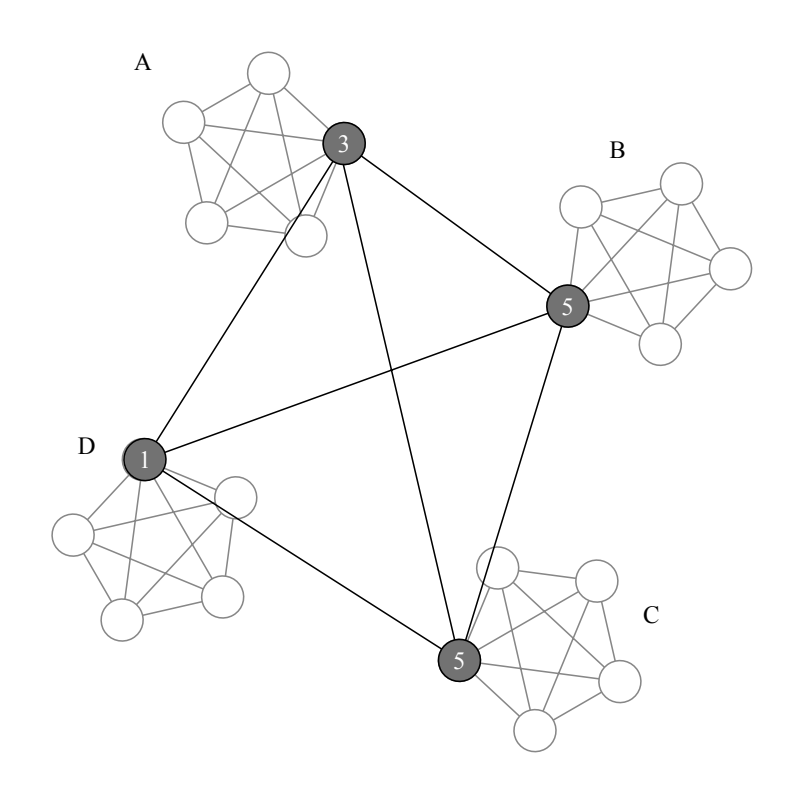
\includegraphics[scale=0.6]{images/cpso_leader_conference.png}
	\label{fig:cpso_leader_conference}
\end{figure}

Quando todos os líderes forem definidos é criado uma nova população somente com eles e acontece mais uma etapa de evolução, atualizando a velocidade e a posição deles uma segunda vez nessa iteração, como é mostrado na Figura \ref{fig:cpso_leader_conference}. Essa etapa de evolução dos líderes é chamado de conferência do líderes (\textit{leader conference}) e tem como objetivo trocar informações entre eles. Por causa dessa última etapa esse algoritmo acaba tendo mais avaliações de \textit{fitness} por ciclo do que o número de indivíduos da população, sendo esse valor mais o número de clãs.

\begin{figure}[!htb]
	\caption{representação dos líderes disseminando a informação}
	\centering
	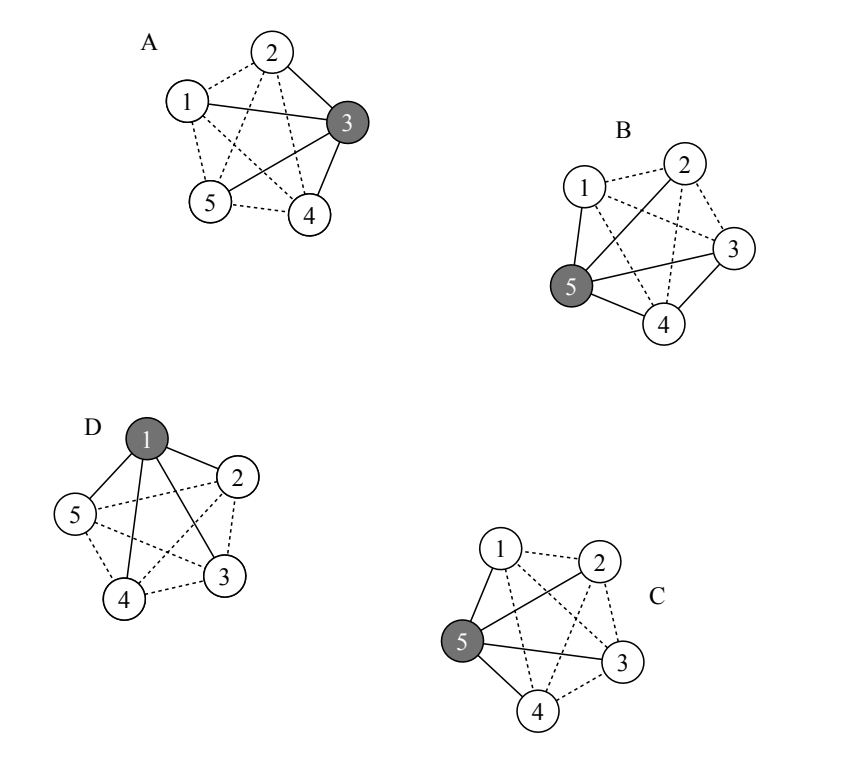
\includegraphics[scale=0.6]{images/cpso_information_sharing.png}
	\label{fig:cpso_information_sharing}
\end{figure}

No começo de cada nova etapa, os líderes de cada clã serão classificados como ótimo global de seus respectivos clãs e poderão disseminar a informação obtida através da conferência dos líderes, como é mostrado na Figura \ref{fig:cpso_information_sharing}. Assim o processo se repete e após cada evolução dos clãs é definido um novo líder.

Um ponto negativo desse processo de separação em clãs, é que existe o risco dessas subpopulações se agruparem, assim perdendo o monitoramento de vários pontos ótimos ao mesmo tempo, e na sua versão padrão não existe uma rotina para evitar isso ou até mesmo dispersar a população, uma vez que foi identificado o agrupamento dos clãs. As etapas do processo de evolução podem ser identificadas no algoritmo \ref{alg:cpso_pseudocode}.

\begin{algorithm}
	\label{alg:cpso_pseudocode}
	InicializarPopulação()\;
	\While{numeroIteração $<=$ totalIterações}{
		\For{clãs}{
			\For{partículas}{
				AtualizarVelocidade()\;
				AtualizarPosição()\;
				CalcularFitness()\;
				AtualizarInformações()\;
			}
			DelegarLider();
		}
		RealizarConferênciaLideres()\;
		numeroIteração ++\;
	}
	\caption{Pseudo-código do Algoritmo de Otimização de Partículas por Clãs}
\end{algorithm}

\section{Diversidade Populacional}
\label{sec:population_diversity}

Uma população com diversidade pode ser capaz de lidar com funções multimodais e explorar simultaneamente diferentes picos na superfície da função objetivo, como também melhorar a exploração global e ajudar a encontrar vários ótimos globais e locais.

Em problemas dinâmicos uma boa diversidade populacional ajuda o sistema a manter um nível satisfatório de \textit{fitness} durante todo o processo de otimização. Ajuda também o sistema a se adaptar as mudanças no ambiente, de forma que, ao perceber essa mudança os indivíduos mais afastados dos pontos ótimos podem encontrar diferentes soluções que podem se tornar novos pontos ótimos.

Além disso, muitos dos problemas dinâmicos possuem mais de um ponto ótimo e algumas estratégias de manutenção da diversidade populacional, mostradas na Seção \ref{sec:maintain_diversity} ajudam a encontrar vários pontos ao mesmo tempo.

\subsection{Manutenção}
\label{sec:maintain_diversity}
As principais estratégias encontradas na literatura são o \textit{fitness sharing, clearing, crowding, deterministic crowding} e \textit{probabilistic crowding}.

Compartilhamento (\textit{Sharing}): Foi introduzido por Goldberg e Richardson \cite{sharing}, com a intenção de localizar múltiplos picos simultaneamente. A ideia básica é punir indivíduos que ocupam as mesmas regiões no espaço de busca por escala a aptidão de cada indivíduo de acordo com o número de indivíduos na vizinhança. Assim, penalizando indivíduos que se aglomeram em conjunto, o regime de partilha impede a convergência para um único pico. O \textit{fitness sharing} de um indivíduo $i$ é definido pela Equação \ref{eq:sharing}. Onde $n$ é o número de indivíduos da população, $\sigma_{share}$ indica o limiar de dissimilaridade e $d_j^i$ é a medida de distância entre o indivíduo $i$ e $j$.

\begin{equation}
\label{eq:sharing}
\begin{split}
& f_{share}^i = \frac{f_i}{\sum_{j=0}^{n} sharing_j^i} \\
& sharing_j^i =
	\begin{cases}
	1 - (d_j^i/\sigma_{share})^2 	& \quad \text{Se } d_j^i < \sigma_{share}\\
	0 							& \quad \text{Se não}\\
	\end{cases}
\end{split}
\end{equation}

Compensação (\textit{clearing}): é um método similar ao Compartilhamento, porém é baseado no conceito de recursos limitados no ambiente \cite{clearing}. Ao invés de compartilhar recursos entre todos os indivíduos de uma subpopulação, o método de compensação atribui o \textit{fitness} apenas para os melhores indivíduos da subpopulação. Assim, o \textit{clearing} preserva o \textit{fitness} dos $k$ melhores indivíduos do nicho e redefine o \textit{fitness} dos outros que pertencem à mesma subpopulação. Como no método de \textit{sharing}, indivíduos pertencem ao mesmo nicho se sua distância no espaço de busca for menor que um limiar de dissimilaridade $\sigma_s$ (raio de \textit{clearing}). O \textit{clearing} pode ser combinado com estratégias de elitismo para preservar as melhores soluções dos nichos durante gerações.

Aglomeração (\textit{Crowding}): O método de \textit{Crowding} foi proposto por De Jong \cite{crowding}. Este método de nichos de espécies compara um descendente com alguns indivíduos escolhidos aleatoriamente da população atual. O indivíduo mais semelhante será substituído se o descendente oferecer melhor valor de \textit{fitness}. O fator de aglomeração (parâmetro $CF$) é definido como uma pequena parcela da população, o qual é utilizado para controlar o tamanho da amostra. Nesse método existe a possibilidade de se sobrescrever um mesmo indivíduo várias vezes, esse fato se chama erro de substituição que é a principal desvantagem do \textit{Crowding}, além disso, o \textit{Crowding} é propenso a aglomeração de indivíduos ao redor dos picos de soluções ótimas.

Aglomeração Determinística (\textit{Deterministic Crowding}): Para aliviar o problema de erro de substituição, foi introduzido uma melhoria na aglomeração original, que não utiliza o parâmetro do fator de aglomeração. Este método foi chamado aglomeração determinista \cite{deterministic_crowding}. Essa abordagem minimiza o erro de substituição significativamente e restaura a pressão seletiva. No entanto, este método também tem uma desvantagem em que aumenta a perda de nichos devido ao uso de seleção por torneio entre indivíduos semelhantes.

Aglomeração Probabilística (\textit{Probabilistic Crowding}): Para superar o problema da falta ótimos locais foi criado o método de aglomeração probabilística \cite{probabilisti_crowding}. A regra de substituição probabilística é usada para manter uma elevada diversidade na população que substitui indivíduos de menor \textit{fitness} por indivíduos de \textit{fitness} mais elevados de acordo com a sua proporção de \textit{fitness}. O principal problema deste processo é que ele tem uma taxa de convergência muito lenta e baixa capacidade de pesquisa.

Lacuna de Geração (\textit{Generation Gap}): Neste modelo apenas uma parte da população (\textit{generation gap}) se reproduz e morre em cada geração. Deste modo o filho substitui o indivíduo mais similar retirado de uma subpopulação aleatória de tamanho $CF$ (\textit{crowding factor}) da população total.

\subsection{Métricas}
\label{sec:evaluete_diversity}

Para avaliar o estado da diversidade de uma população são utilizados dois tipos de medidas de diversidade: A medida de diversidade fenotípica (MDF) e genotípica (MDG). A MDF mede a diversidade de \textit{fitness} das soluções, ou seja, a diversidade de diferentes qualidades de soluções. Já a MDG mensura a diversidade genética das soluções, avaliando o conjunto de variáveis (genes) que influenciam na função objetivo.

A MDF é apresentada na equação \ref{eq:fenotype}, em que variável $VMD$ é um fator de normalização que corresponde a medida de diversidade de uma população virtual com os valores de \textit{fitness} distribuídos de maneira uniforme com uma distância predeterminada. Onde $f_{worst}$ representa o pior \textit{fitness} e o $f_{best}$ o melhor \textit{fitness} e $N$ o tamanho da população \cite{phenotypic}. Quando o tamanho da população ou a faixa de \textit{fitness} absoluto são modificados é necessário recalcular o $VMD$. É importante ressaltar que para calcular a MDF é preciso que os valores de \textit{fitness} estejam ordenados.

\begin{equation}
\label{eq:fenotype}
\begin{split}
& MDF = \frac{\sum_{i=0}^{n-1} \ln(1 + |f_i - f_{i+1}|)}{VMD} \\
\end{split}
\end{equation}

A MDG  proposta por Corriveau \cite{genotypic}. Esta medida foi desenvolvida com base na MDF, sendo indicada para variáveis contínuas. A medida é apresentada na Equação \ref{eq:genotypic}, onde $D$ é a quantidade de dimensões da solução, $N$ o tamanho da população e $x$ a solução candidata. A variável
$NMDF$ é o fator de normalização que corresponde ao valor máximo de diversidade conhecida até o momento. O valor 1 obtido da medida corresponde a diversidade genotípica máxima enquanto o valor 0 corresponde a convergência da população de soluções.

\begin{equation}
\label{eq:genotypic}
MDG = \frac{\sum_{i=0}^{n-1} \ln \left(1 + \min_{j \in [i_1,N]} \frac{1}{D} \sqrt{ \sum\limits_{k=1}^{D} (x_{i,k} - x_{j,k})^2}\right)}{NMDF}
\end{equation}

\section{Aplicação do AG em ambientes dinâmicos}
\label{sec:ag_behaviour}

Um trabalho que pode ser citado em relação a avaliação de algoritmos em ambientes dinâmicos é o trabalho de \cite{rand2005measurements}, em que é feita uma análise do comportamento do AG em um ambientes dinâmicos discreto. Mesmo sendo um trabalho que é aplicado em uma classe de problemas diferente da abordada por este trabalho, ele mostra que na maioria dos trabalhos que analisam um algoritmo somente avaliam o desempenho, ou seja, o quão perto do melhor resultado chegou. São analisados quatro fatores principais para determinar a eficiência do AG em ambientes dinâmicos, sendo eles:

\begin{enumerate}
	\item Desempenho: Para entender o desempenho do algoritmo existem duas vertentes, sendo uma a avaliação do melhor indivíduo da população para cada iteração do AG, e a outra é avaliar a média da população em para cada uma das iterações. Para a aplicar AG no SL-HDF é usado a melhor solução antes da primeira alteração como média inicial.

	\item Satisfatibilidade: É a medida da habilidade do sistema de manter um certo nível de \textit{fitness} no decorrer da otimização e não deixar esse nível cair abaixo de um determinado limite. Esta medida não necessariamente representa o quão rápido (menos interações necessárias) o sistema chega em uma nova ótima solução, e sim se ele consegue manter um nível de \textit{fitness} da população.

	\item Robustez: É a medida de como o sistema reage a uma alteração, de forma que ao sofrer uma alteração o \textit{fitness} não pode ter uma queda muito brusca. A medida de robustez usada neste trabalho foi a média do \textit{fitness} no estado atual do ambiente sobre a média do \textit{fitness} no estado anterior do sistema, para uma alteração perceptível.

	\item Diversidade: É a medida que representa a variação do genoma da população, de forma que uma população que possui uma alta diversidade tem maiores chances de encontrar novas solução e assim se adaptar melhor a uma mudança do ambiente. Existem várias técnicas estudadas para manter a diversidade da população durante o processo evolutivo, e para medir a diferença genotípica é usado a distância de \textit{Hamming}.
\end{enumerate}

Na aplicação do AG pode-se notar que a performance do algoritmo no ambiente dinâmico é superior sua aplicação em ambientes estáticos quando há um grande número de iterações. Inicialmente o ambiente dinâmico perde para o estático mas a partir da metade do processo evolutivo o dinâmico gera um \textit{fitness} maior no melhor indivíduo e na média da população.

A análise da satisfatibilidade mostra o nível do \textit{fitness} durante o processo evolutivo, e com ele pode-se notar que mesmo em relação a uma aplicação em um ambiente estático, o nível de \textit{fitness} pode ser mantido acima de um limiar.

Na análise de robustez pode-se notar que a cada mudança no ambiente existe uma queda na média do \textit{fitness}, porém o sistema se recupera rapidamente, e a cada nova mudança e queda do \textit{fitness} diminui.

A diversidade do sistema teve um comportamento inesperado, pois inicialmente achava-se que o sistema iria perder a diversidade até uma mudança ocorrer e depois a diversidade iria aumentar, porém aconteceu exatamente o contrário, tendo que após uma mudança a diversidade diminui e vai aumentando até identificar uma nova mudança.

\section{Problemas Dinâmicos com Domínio Contínuo}
\label{sec:problemas}
Neste capítulo é apresentado uma breve introdução aos \textit{benchmarks} que serão utilizados para análise nesse trabalho, junto a isso é feita uma introdução aos problemas dinâmicos, suas variações e dificuldades.

Durante o dia a dia, pode-se observar diversos problemas complexos em que as condições do ambiente podem mudar com o tempo, sendo assim uma solução válida encontrada em um instante anterior acaba não sendo mais suficientemente boa para suprir as necessidades das novas condições \cite{branke2012evolutionary}. Para problemas com mudanças em seu ambiente é necessário um sistema de resolução que se adapte as alterações e esteja sempre apto a procurar por soluções melhores. Na computação existem várias áreas nas quais se dedicam a otimizar esses problemas, como por exemplo os EA e os SI. Para poder avaliar os algoritmos utilizados na otimização destes problemas são geradas funções \textit{benchmarks} que apresentam características dos problemas reais, como por exemplo mudança de elevação de terrenos.

\section{Funções \textit{Benchmark}}
\label{sec:revisao_benchmark}
O uso das funções \textit{benchmark} é um ponto crucial para o desenvolvimento, comparação, avaliação e otimização dessa classe de problemas \cite{evolution_dynamic}. O fato das condições do problema variarem de acordo com o tempo acrescenta uma camada de dificuldade a mais para obter uma solução satisfatória após uma mudança. Um bom \textit{benchmark} deve possuir as seguintes características.

\begin{enumerate}  
	\item Flexibilidade: Configurável sobre diferentes abordagens dinâmicas, como por exemplo, a frequência ou intensidade das alterações no ambiente, em diferentes escalas.
	
	\item Simplicidade e Eficiência: Deve ser fácil de implementar e analisar.
	
	\item Associação com Problemas Reais: Ter a capacidade de fazer previsões em problemas reais ou se assemelhar em alguma extensão.
\end{enumerate}

Para a analisar um \textit{benchmark} é necessário dar atenção para o tipo de dinamismo que esse problema apresenta, pois para otimizá-lo são escolhidas estratégias de otimização baseadas no tipo de dinamismo. Cada \textit{benchmark} possui suas características e com isso cada algoritmo aplicado a ele terá que analisar como está abordando essas peculiaridades. As Características observadas nas funções encontradas são \cite{cruz2011optimization}:

\begin{enumerate}
	\item Influência Temporal: Sempre que uma solução futura depende de outra encontrada anteriormente pelo algoritmo, ou seja, quando o tipo de mudança que o algoritmo vai sofrer depende de quais soluções foram encontradas ao decorrer da otimização. Neste caso os resultados podem mudar para cada tentativa de otimização.
	
	\item Previsibilidade: Quando as mudanças geradas pelo problema seguem um padrão que pode ser previsto durante a otimização do problema. Podem ser alterações por mudança em uma escala fixa, incremental, cíclica ou periódica.
	
	\item Visibilidade: Sempre que as mudanças do ambiente são visíveis pelo algoritmo otimizando o problema. O algoritmo não deve precisar utilizar muitos detectores para perceber a mudança no ambiente, podem ser pontos específicos do espaço, que são detectados ao reavaliar a função objetivo, ou até mesmo, as restrições.
	
	\item Problemas com Restrições: As mudanças do problema podem ocorrer nas restrições, que podem mudar ao longo do tempo (a variável de tempo influencia na função de restrição) ou podem ser ativadas e/ou desativadas durante a otimização.
	
	\item Número de Objetivos: São os problemas multiobjetivos, que neste caso podem alterar o número de objetivos durante a otimização, chegando até, ao ponto de ter somente um objetivo em vista.
	
	\item Intensidade das Mudanças: Indica qual a escala da mudança, ou seja, quão expressiva é está alteração em relação ao \textit{fitness} do indivíduo, tendo como preocupação o limite das mudanças.
	
	\item Fator da Mudança: Onde o dinamismo pode ocorrer, sendo na função objetivo, no domínio das variáveis no número de variáveis, nas restrições ou outros parâmetros.  
\end{enumerate}

\subsection{Avaliação de Desempenho}
\label{sec:perfermance_measures}

Para avaliar um \textit{benchmark} são estipuladas métricas que serão utilizadas para medir a qualidade dos resultados obtidos pelo algoritmo de otimização. Os métodos de avaliação apresentados foram selecionados por serem amplamente utilizados em algoritmos bioinspirados aplicados em ambientes dinâmicos e serão usados para avaliar o desempenho dos algoritmos selecionados neste trabalho.
A forma de avaliação pode ser dividida em dois grandes grupos: Medida de desempenho baseados em otimalidade e em comportamento.

\subsubsection{Otimalidade}
As medidas de desempenho baseadas na otimalidade avaliam a capacidade dos algoritmos em encontrar as soluções com o melhor valor de \textit{fitness} ou as que estão mais próximas do ótimo global (medidas baseadas na distância) e essa avaliação leva em conta o algoritmo como um todo. Entre elas tem-se:

\begin{itemize}
	\item Melhor da Geração: Avalia qual o melhor indivíduo de cada iteração do algoritmo, gerando assim uma curva de desempenho que apresenta os pontos de melhora do algoritmo e o quão perto está do ótimo do problema. Esse é o método mais frequentemente utilizado.
	
	\item Melhor Erro Antes da Mudança: Calcula a média do erro (diferença da melhor solução atual para o ótimo do problema) da população logo antes da mudança do ambiente. Este caso só pode ser usado quando o dinamismo do \textit{benchmark} gerado é previsível ou facilmente identificável, que por sua vez, dependo de como o \textit{benchmark} muda o ambiente.
	
	\item Pontuação Normalizada: Mede a diferença entre uma determinada gama de algoritmos em relação a uma lista predeterminada de problemas, fazendo com que cada algoritmo execute cada problema um número determinado de vezes. Com os resultados normalizados, para a melhor solução é atribuído o valor 1 (um) e para a pior solução é atribuído o valor 0 (zero).
\end{itemize}

Para quantificar a otimalidade é utilizado o \textit{Offline Error} (OFFE) \cite{offlineError}, que representa o quanto o algoritmo chegou perto do ponto ótimo. Essa métrica é usada pois nos \textit{benchmarks} os valores de \textit{fitness} gerados, são diferentes para cada execução, sendo assim, com o valor de \textit{Offline Error} pode-se estipular uma aproximação para cada execução em média. O cálculo dessa métrica é feito pela diferença do melhor da população.

\begin{equation}
\label{eq:offline_error}
\begin{split}
& OFFE = fitness_{best} - population_{best} \\
\end{split}
\end{equation}

Onde o $fitness_{best}$ é o objetivo da função avaliada e o $population_{best}$ é o melhor resultado encontrado pela população até agora.

\subsubsection{Comportamento}
As medidas de desempenho baseadas em comportamento avaliam a influência de certos comportamentos que são importantes na hora de manter um nível de \textit{fitness}, como por exemplo:

\begin{itemize}
	\item Manutenção da Diversidade: Como o nome já diz, mede quanto que um comportamento pode ajudar na manutenção da diversidade da população ao longo do processo de otimização. Este é um fator muito estudado em ambientes dinâmicos, pois com uma grande diversidade da população existem mais chances de se encontrarem os novos ótimos globais.
	
	\item Velocidade de Convergência Após uma Mudança: Mede quão rápido o sistema se adapta após perceber uma alteração. Essa medida de comportamento não se aplica a sistemas que tem dificuldades em perceber uma alteração no ambiente. Para analisar essa medida é feita uma análise de quantas iterações são necessárias para se encontrar um novo ótimo, em relação a distância.
	
	\item Performance Após uma Mudança: Mede a capacidade do algoritmo de buscar novos resultados após as mudanças no ambiente, de forma que restringe a queda do \textit{fitness} quando percebe uma piora. Essa medida também é conhecida como medida de estabilidade ou satisfatibilidade.
\end{itemize}

\section{Instâncias de Problemas}
\label{sec:revisao_dinamic_problems}
Nesta etapa são apresentados e detalhados os problemas que serão abordados no trabalho. Os problemas selecionados para esse trabalho serão usados para realizar uma análise comparativa com outras abordagens encontradas na literatura e também testar o desempenho de cada operador evolutivo que os algoritmos irão abordar. A maioria dos problemas selecionados não possui um \textit{link} temporal com as soluções anteriores. São apresentados com e sem restrições na função objetivo ou no limite do domínio das variáveis, tendo em sua maioria dinamismos previsíveis, periódicos e constantes.

\subsection{\textit{Moving Peaks} - MP}
\label{sec:moving_peaks}

O \textit{benchmark} de movimentação de picos (\textit{moving peaks}) foi desenvolvido por Jürgen Branke \cite{moving_peak_1999} e tem como principal ideia gerar um problema que possa ser amplamente utilizado em algoritmos bioinspirados. A característica diferencial do MP em relação a maioria dos problemas dinâmicos, até o dado momento, é que eles sofriam uma alteração drástica que gerava um novo ambiente totalmente diferente do anterior, tornando assim um recomeço da otimização uma solução melhor.

A ideia é gerar um \textit{benchmark} que, ao sofrer uma mudança no ambiente, ficasse levemente alterado, o suficiente para que as soluções anteriores ajudassem a encontrar as novas geradas. Para isso foi criado o \textit{moving peaks} com a ideia de ter uma paisagem multidimensional artificial que consiste em vários picos, em que a altura, a largura e a posição de cada pico é ligeiramente alterada cada vez que uma mudança no ambiente ocorre.

A função objetivo é dada pela Equação \ref{eq:moving_peak_equacion}, na qual tem-se $ H $ como altura, $ W $ como peso, $ n $ como o número de picos e $ m $ como o número de dimensões. Todos esses parâmetros são definidos previamente aos testes.

\begin{equation}
\label{eq:moving_peak_equacion}
F(\vec{x},t) = \max_{i = 1 \to n} \frac {H_i(t)}{1 + W_i(t)\sum_{j=1}^{m} (x_j - X_j(t))^2}
\end{equation}

A cada $\Delta e$ (valor que representa o intervalo/frequência das mudanças do ambiente), a altura e o peso são alterador adicionando uma variável aleatória. O local de cada um dos picos é movido por um vetor $\vec{v}$ a uma distância $ s $ fixa para uma direção aleatória. Essas alterações podem ser descritas pela Equação \ref{eq:moving_peak_alterations}.

\begin{equation}
\label{eq:moving_peak_alterations}
\begin{split}
& \sigma \in N(0,1) \\
& H_i(t) = H_i(t-1) + 7.\sigma \\
& W_i(t) = W_i(t-1) + 0,01.\sigma \\
& \vec{X}_i(t) = \vec{X}_i(t-1) + \vec{v}
\end{split}
\end{equation}

Um exemplo de como as máximas se movem ao longo do tempo em um espaço bidimensional pode ser visto na Figura \ref{fig:moving_peaks}

\begin{figure}[!htb]
	\caption{Gráfico de duas dimensões do movimento dos picos, após 300 alterações no ambiente, $ s = 0,9 $}
	\centering
	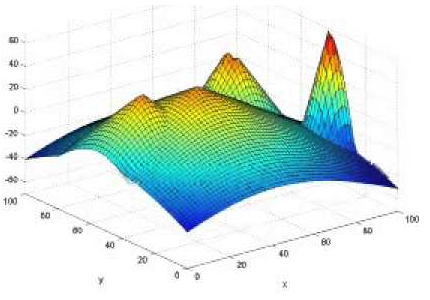
\includegraphics[scale=0.5]{images/moving_peak.png}
	\label{fig:moving_peaks}{\\Fonte: \citeonline{moving_peak_1999}.}
\end{figure}

\subsection{\textit{Ocillating Peaks} - OP}
\label{sec:ocillating_peaks}

O \textit{benchmark} de oscilação de picos (\textit{ocillating peaks}) é baseado no de movimentação de picos, porém foi desenvolvido para algoritmos evolutivos com utilização de memória.

É uma combinação linear entre duas funções em que o peso delas se alteram ao longo do tempo, portanto, a função $G$, começa em $g_1$, passa para $g_2$, depois volta para $g_1$ e assim sucessivamente. Em outras palavras, o máximo absoluto de $G$ oscila entre dois pontos $g_1$ e $g_2$. As funções que representam as alterações da função $G$ estão representadas na Equação \ref{eq:ocillating_peak_alterations}, em que, $\lambda (t)$ representa a oscilação da função, $n$ é a soma dos picos das duas funções que compõem a combinação linear e $m$ é o número de dimensões.

\begin{equation}
\label{eq:ocillating_peak_alterations}
\begin{split}
& \delta \in N(0,1) \\
& \lambda (t) = \frac{\cos{\frac{2\pi t}{100\delta}} +1}{2} \\
& g_1(\vec{x}) = \sum_{i=1}^{n/_2} \frac{H_i}{1+W_i \sum_{j=1}^{m} (x_j - X_j(t))^2} \\
& g_2(\vec{x}) = \sum_{i=n/_2+1}^{n} \frac{H_i}{1+W_i \sum_{j=1)}^{m} (x_j - X_j(t))^2} \\
& G(t,\vec{x}) = \lambda (t) g_1(\vec{x}) + (1-\lambda (t))g_2(\vec{x})
\end{split}
\end{equation}

\subsection{Gerador de Problemas de teste para Ambientes não Estacionários}
\label{sec:df1_generator}

O Gerador de Problemas de testes para Ambientes não Estacionários (DF1) foi utilizado para gerar ambientes, tais como o mostrado na Figura \ref{fig:problem_generator} proposto por Morrison e Jong \cite{morrison1999test}. Este gerador é capaz de criar um número especificado de pontos ótimos em duas dimensões utilizando a Equação \ref{eq:problem_generator} 

\begin{figure}[!htb]
	\caption{Gráfico que representa os ambientes gerados pelo Gerador de Problemas testes para Ambientes não Estacionários}
	\centering
	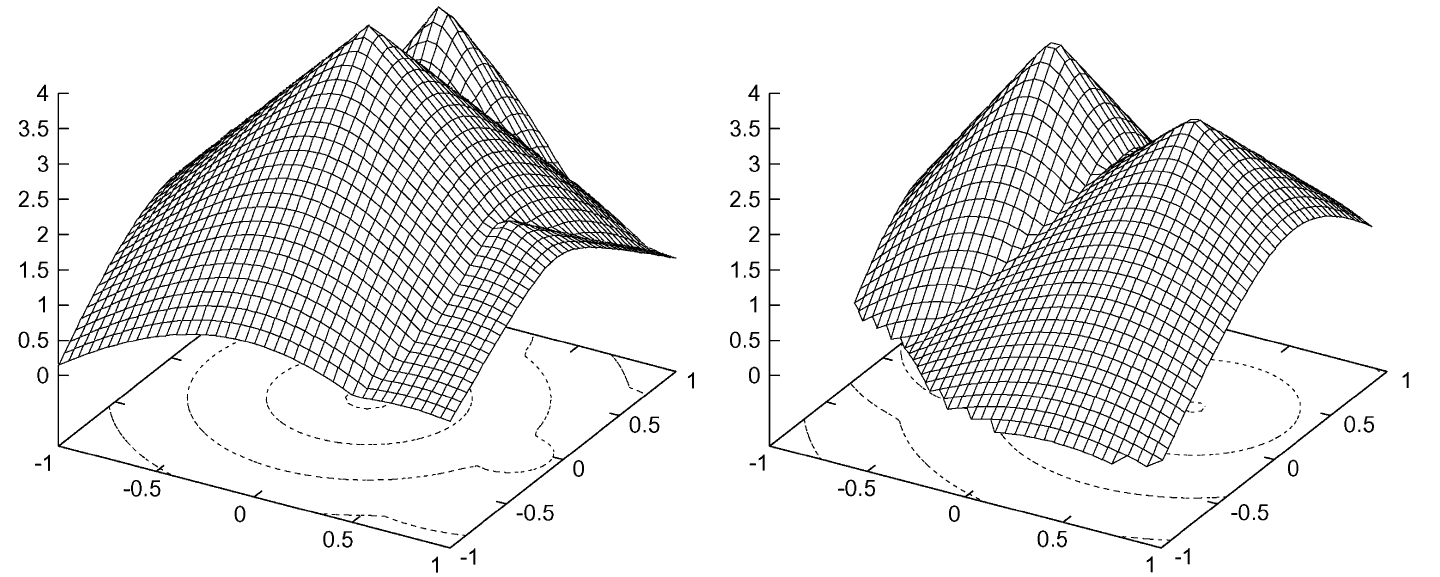
\includegraphics[scale=0.31]{images/bm_generator.png}
	\label{fig:problem_generator}{\\Fonte: \citeonline{morrison1999test}.}
\end{figure}

\begin{equation}
\label{eq:problem_generator}
\begin{split}
& f(X,Y) = \max_{i=1,N}\left[H_i - R_i . \sqrt{(X - X_i)^2 + (Y - Y_I)^2}\right] \\
& H_i \in [H_{base}, H_{base} + H_{range}] \\
& R_i \in [R_{base}, R_{base} + R_{range}]
\end{split}
\end{equation}

\noindent Em que $N$ representa o número de pontos ótimos a serem gerados, $(X,Y)$ representa sua posição, $H_i$ representa sua altura e $R_i$ representa sua inclinação. o limite da altura e inclinação são apresentados na Equação \ref{eq:problem_generator}. Nesse sistema variam suas posições, formas e altura. A altura varia entre um valor máximo e mínimo, criando assim um perfil de dente de serra, enquanto a altura é representada graficamente. O \textit{fitness} de cada ponto da superfície é atribuído a altura máxima de todos os pontos ótimos.

Embora o número de pontos ótimos presente não possa ser alterado uma vez que o ambiente tenha sido inicializado, a combinação da mudança altura e posições faz com uma solução ótima fique temporariamente obscura em relação aos vizinhos. Esse fenômeno gera a impressão que alguns pontos desaparecem e ressurgem, porém a quantidade de picos não é alterada. O dinamismo do ambiente pode ser especificado por um parâmetro $A$ que varia de [0, 4]. A direção de cada etapa é escolhida aleatoriamente para coordenadas espaciais, com paços que podem colocar um pico fora dos limites das variáveis. A direção da mudança nas variáveis de altura e inclinação são escolhidas aleatoriamente inicialmente e continuam nessa direção até exceder o intervalo.